%
% $File: report.tex
% $Date: Fri Dec 27 22:07:14 2013 +0800
%

\documentclass{article}
\usepackage{fontspec}
\usepackage{zhspacing,url,amsmath,amssymb,verbatim}
\usepackage{pdfpages}
\zhspacing
\usepackage{listings}
\usepackage[hyperfootnotes=false,colorlinks,linkcolor=blue,anchorcolor=blue,citecolor=blue]{hyperref}
\usepackage[backend=biber]{biblatex}
\usepackage{graphicx}
\usepackage{minted}
\usepackage{subfigure}
\usepackage{indentfirst}
\usepackage{cases}
\usepackage{environ}
\usepackage{array}
\usepackage[top=1in, bottom=1in, left=1.25in, right=1.25in]{geometry}
\usepackage{caption}
%\usepackage{tikz}
%\usepackage{dot2texi}

% $File: mint-defs.tex
% $Date: Sun Nov 17 23:37:24 2013 +0800
% $Author: Xinyu Zhou <zxytim@gmail.com>

\newcommand{\inputmintedConfigured}[3][]{\inputminted[fontsize=\footnotesize,
	label=#3,linenos,frame=lines,framesep=0.8em,tabsize=4,#1]{#2}{#3}}

\newcommand{\txtsrc}[2][]{\inputmintedConfigured[#1]{text}{#2}}
\newcommand{\txtsrcpart}[4][]{\txtsrc[firstline=#3,firstnumber=#3,lastline=#4,#1]{#2}}

\newcommand{\cppsrc}[2][]{\inputmintedConfigured[#1]{cpp}{#2}}
\newcommand{\cppsrcpart}[4][]{\cppsrc[firstline=#3,firstnumber=#3,lastline=#4,#1]{#2}}

\newcommand{\javasrc}[2][]{\inputmintedConfigured[#1]{java}{#2}}
\newcommand{\javasrcpart}[4][]{\javasrc[firstline=#3,firstnumber=#3,lastline=#4,#1]{#2}}

\newcommand{\matlabsrc}[2][]{\inputmintedConfigured[#1]{matlab}{#2}}
\newcommand{\matlabsrcpart}[4][]{\matlabsrc[firstline=#3,firstnumber=#3,lastline=#4,#1]{#2}}

\newcommand{\pysrc}[2][]{\inputmintedConfigured[#1]{matlab}{#2}}
\newcommand{\pysrcpart}[4][]{\matlabsrc[firstline=#3,firstnumber=#3,lastline=#4,#1]{#2}}

%\usepackage[T1]{fontenc}
\usepackage{lmodern}
\usepackage{amssymb,amsmath}
\usepackage{ifxetex,ifluatex}
\usepackage{fixltx2e} % provides \textsubscript
% use upquote if available, for straight quotes in verbatim environments
\IfFileExists{upquote.sty}{\usepackage{upquote}}{}
\ifnum 0\ifxetex 1\fi\ifluatex 1\fi=0 % if pdftex
  \usepackage[utf8]{inputenc}
\else % if luatex or xelatex
  \usepackage{fontspec}
  % commented by Xinyu Zhou
  \ifxetex
    \usepackage{xltxtra,xunicode}
  \fi
  \defaultfontfeatures{Mapping=tex-text,Scale=MatchLowercase}
  \newcommand{\euro}{€}
\fi
% use microtype if available
\IfFileExists{microtype.sty}{\usepackage{microtype}}{}
\usepackage{color}
\usepackage{fancyvrb}
\newcommand{\VerbBar}{|}
\DefineShortVerb[commandchars=\\\{\}]{\|}
\DefineVerbatimEnvironment{Highlighting}{Verbatim}{commandchars=\\\{\}}
% Add ',fontsize=\small' for more characters per line
\newenvironment{Shaded}{}{}
\newcommand{\KeywordTok}[1]{\textcolor[rgb]{0.00,0.44,0.13}{\textbf{{#1}}}}
\newcommand{\DataTypeTok}[1]{\textcolor[rgb]{0.56,0.13,0.00}{{#1}}}
\newcommand{\DecValTok}[1]{\textcolor[rgb]{0.25,0.63,0.44}{{#1}}}
\newcommand{\BaseNTok}[1]{\textcolor[rgb]{0.25,0.63,0.44}{{#1}}}
\newcommand{\FloatTok}[1]{\textcolor[rgb]{0.25,0.63,0.44}{{#1}}}
\newcommand{\CharTok}[1]{\textcolor[rgb]{0.25,0.44,0.63}{{#1}}}
\newcommand{\StringTok}[1]{\textcolor[rgb]{0.25,0.44,0.63}{{#1}}}
\newcommand{\CommentTok}[1]{\textcolor[rgb]{0.38,0.63,0.69}{\textit{{#1}}}}
\newcommand{\OtherTok}[1]{\textcolor[rgb]{0.00,0.44,0.13}{{#1}}}
\newcommand{\AlertTok}[1]{\textcolor[rgb]{1.00,0.00,0.00}{\textbf{{#1}}}}
\newcommand{\FunctionTok}[1]{\textcolor[rgb]{0.02,0.16,0.49}{{#1}}}
\newcommand{\RegionMarkerTok}[1]{{#1}}
\newcommand{\ErrorTok}[1]{\textcolor[rgb]{1.00,0.00,0.00}{\textbf{{#1}}}}
\newcommand{\NormalTok}[1]{{#1}}
% \ifxetex
%   \usepackage[setpagesize=false, % page size defined by xetex
%               unicode=false, % unicode breaks when used with xetex
%               xetex]{hyperref}
% \else
%   \usepackage[unicode=true]{hyperref}
% \fi
\hypersetup{breaklinks=true,
            bookmarks=true,
            pdfauthor={},
            pdftitle={},
            colorlinks=true,
            urlcolor=blue,
            %linkcolor=magenta,
            pdfborder={0 0 0}}
%\urlstyle{same}  % don't use monospace font for urls
\setlength{\parindent}{0pt}
\setlength{\parskip}{6pt plus 2pt minus 1pt}
\setlength{\emergencystretch}{3em}  % prevent overfull lines
%\setcounter{secnumdepth}{0}



\newcommand{\figref}[1]{\hyperref[fig:#1]{Fig.\ref*{fig:#1}}}
\newcommand{\tableref}[1]{\hyperref[table:#1]{Table.\ref*{table:#1}}}
\newcommand{\centerize}[1]{\begin{center} #1 \end{center}}
\newcommand{\secref}[1]{\hyperref[sec:#1]{Section.\ref*{sec:#1}}}
\newcommand{\appref}[1]{\hyperref[app:#1]{App.\ref*{app:#1}}}


\newcommand{\cmd}[1]{{\it #1}}
\newcommand{\ccmd}[1]{\centerize{\cmd{#1}}}

\title{Digital Signal Processing: Speaker Recognition \\ Stage Report}
\author{Xinyu Zhou, Yuxin Wu, and Tiezheng Li\\ Tsinghua University}
\date{}

\bibliography{refs.bib}
\begin{document}

\fontsize{11pt}{1.4em}
\setlength{\baselineskip}{1.6em}
\maketitle

%File: intro.tex
%Date: Fri Jan 03 22:40:59 2014 +0800
%Author: Yuxin Wu <ppwwyyxxc@gmail.com>


\section{Introduction}
\textbf{Speaker recognition} is the identification of the person who is speaking by characteristics
of their voices (voice biometrics), also called voice recognition. \cite{SRwiki}

A \textbf{Speaker Recognition} tasks can be classified with respect to different criterion:
Text-dependent or Text-independent, Verification (decide whether the person is he claimed to be) or
Identification (decide who the person is by its voice).\cite{SRwiki}

Speech is a kind of complicated signal produced as a result of several transformations occurring at
different levels: semantic, linguistic and acoustic.
Differences in these transformations may lead to differences in the acoustic properties of the signals.
The recognizability of speaker can be affected not only by the linguistic message
but also the age, health, emotional state and effort level of the speaker.
Background noise and performance of recording device also interfere
the classification process.

Speaker recognition is an important part of Human-Computer Interaction (HCI).
As the trend of employing wearable computer reveals,
Voice User Interface (VUI) has been a vital part of such computer.
As these devices are particularly small, they are more likely to lose and be stolen.
In these scenarios, speaker recognition is not only a good HCI,
but also a combination of seamless interaction with computer and security guard
when the device is lost.
The need of personal identity validation will become more acute in the future.
Speaker verification may be essential in business telecommunications.
Telephone banking and telephone reservation services will develop rapidly
when secure means of authentication were available.

Also,the identity of a speaker is quite often at issue in court cases.
A crime victim may have heard but not seen the perpetrator,
but claim to recognize the perpetrator as someone whose voice was previously familiar;
or there may be recordings of a criminal whose identity is unknown.
Speaker recognition technique may bring a reliable scientific determination.

Furthermore, these techniques can be used in environment which demands high security.
It can be combined with other biological metrics to form a multi-modal authentication system.

In this task, we have built a proof-of-concept text-independent speaker recognition system with
GUI support. It is fast, accurate based on our tests on large corpus.
And the gui program only require very short utterance to quickly respond.
The whole system is fully described in this report.
This project is developed at Git9\footnote{Git hosting service of the department of CST, Tsinghua Univ., currently maintained by Yuxin Wu. See
  \url{http://git.net9.org}},
and is also hosted on github\footnote{See \url{https://github.com/ppwwyyxx/speaker-recognition}}.
The repository contains the source code, all documents, experiment log, as well as a video demo.
The complete pack of this project also contains all the intermediate data, models, recordings, and 3rd party libraries.



\section{Approach}
The task of speaker recognition can be considered as a task of classification. Thus a number of machine learning techniques
can be applied to this task. In general, this task should cover the following three topics:

\begin{enumerate}
  \item Feature Extraction: process the voice signal and extract acoustic features that
	  could describe the acoustic characteristics of speakers, which can be correlated
	  in some extend to model latter used.

  \item Acoustic Model: provide the functionality of registration as well as identification or verification.

  \item Evaluation: Evaluate our approach using datasets with appropriate metrics.
\end{enumerate}

\subsection{Feature Extraction}
The task of speaker recognition is highly correlated to the task of speech recognition.
In the field of speech recognition, Complex Cepstrum \cite{cepstrum} is
considered to be a concise description to the original acoustic signal.
In particular, Mel-frequency Cepstral Coefficients (MFCC), is a state-of-the-art standard feature
widely used in Automatic Speech Recognition (ASR) system.
The general procedure for calculating MFCC is as follows:
\begin{figure}[H]
  \centering
  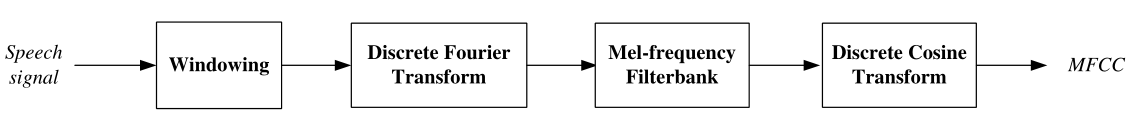
\includegraphics[width=\textwidth]{res/MFCC.png}
\end{figure}

As for speaker recognition, several different features are suggested and compared
by researchers \cite{evaluation}. Cepstrum still proves to be a robust and effective
feature in this task. Therefore, a bunch of cepstral features, including MFCC,
LPCC (Linear Prediction Cepstrum Coefficients), are commonly used
in speaker recognition system.\cite{feature}

We plan to implement common cepstral features used by researchers, and use a
combination of some of them, according to the further observation and test on how
much they contribute to the task.

\subsection{Model}
According to works in years, Gaussian Mixture Model (GMM)
has been a common approach to acoustic modeling.\cite{GMM}
GMM can be used to acquire an acoustic model $P(\mathbf{O} | \mathbf{W}) $,
which gives the probability of a given observation
$\mathbf{O}$ under certain word $\mathbf{W}$. By using GMM, this
conditional probability can be well estimated by modeling the distribution as
a sum of several normal distribution.

In addition to that, Hidden Markov Model (HMM) is a main-stream approach in ASR system,
since it can describe sequential relation of observations.\cite{SLP}
We have noticed a few research-oriented open-source speech recognition
tool building on HMM, such as HTK\cite{htk}.
Such tools might be quite useful in buiding a speaker recognition system.

Recently, some common machine learning model are also applied to the task of speaker
recognition. \cite{svm} suggested a method of using SVM in speaker recognition.
Deep neural networks are also used in speech processing recently.\cite{deep}

HMM and GMM will probably be our first attempt, as they are already widely used and proven to be
efficient and effective.  We might also try to migrate our extracted feature to
some other available models.

\subsection{Evaluation}
\subsubsection{Dataset}
There are a number of well-known databses for speaker recognition system evaluation,
such as KING speaker verification\cite{king}. \cite{database} gives description on
several common databases. But most of these databases are not free of charge.
We intend to search for an freely available database,
otherwise we have to build some simple test cases by our own.
\subsubsection{Metrics}
As we intend to distinguish different speakers, the primary goal is overall
accuracy of the system we built. Furthermore, the performance may differ from
speaker to speaker, which may provide with additional feedback to our approach.
Thus we shall examine precision, recall and $F_1$ score for each speaker.


\section{Performance}
\label{sec:result}
We have tested our approaches under various parameters, based on a corpus described in \secref{data}.

All the tests in this section have been conducted serval times
(depending on computation cost, vary from 10 to 30)
with random selected training and testing speakers.
The average over these tests are considered as confidential result.

\subsection{Efficiency Test of our GMM}
We have extensively examined the efficiency of our implementation of GMM
compared to scikit-learn version. Test is conducted using real MFCC data with
13 dimensions, 20ms frame length. We consider the scenario when training a UBM with 256 mixtures.
We examine the time used for ten iteration.  For comparable results, we diabled
the K-means initialization process of both scikit-learn GMM implementation and
ours. Time used for ten iterations under different data size and concurrency
is recorded.

\begin{figure}[!ht]
	\begin{minipage}{0.48\linewidth}
		\centering
		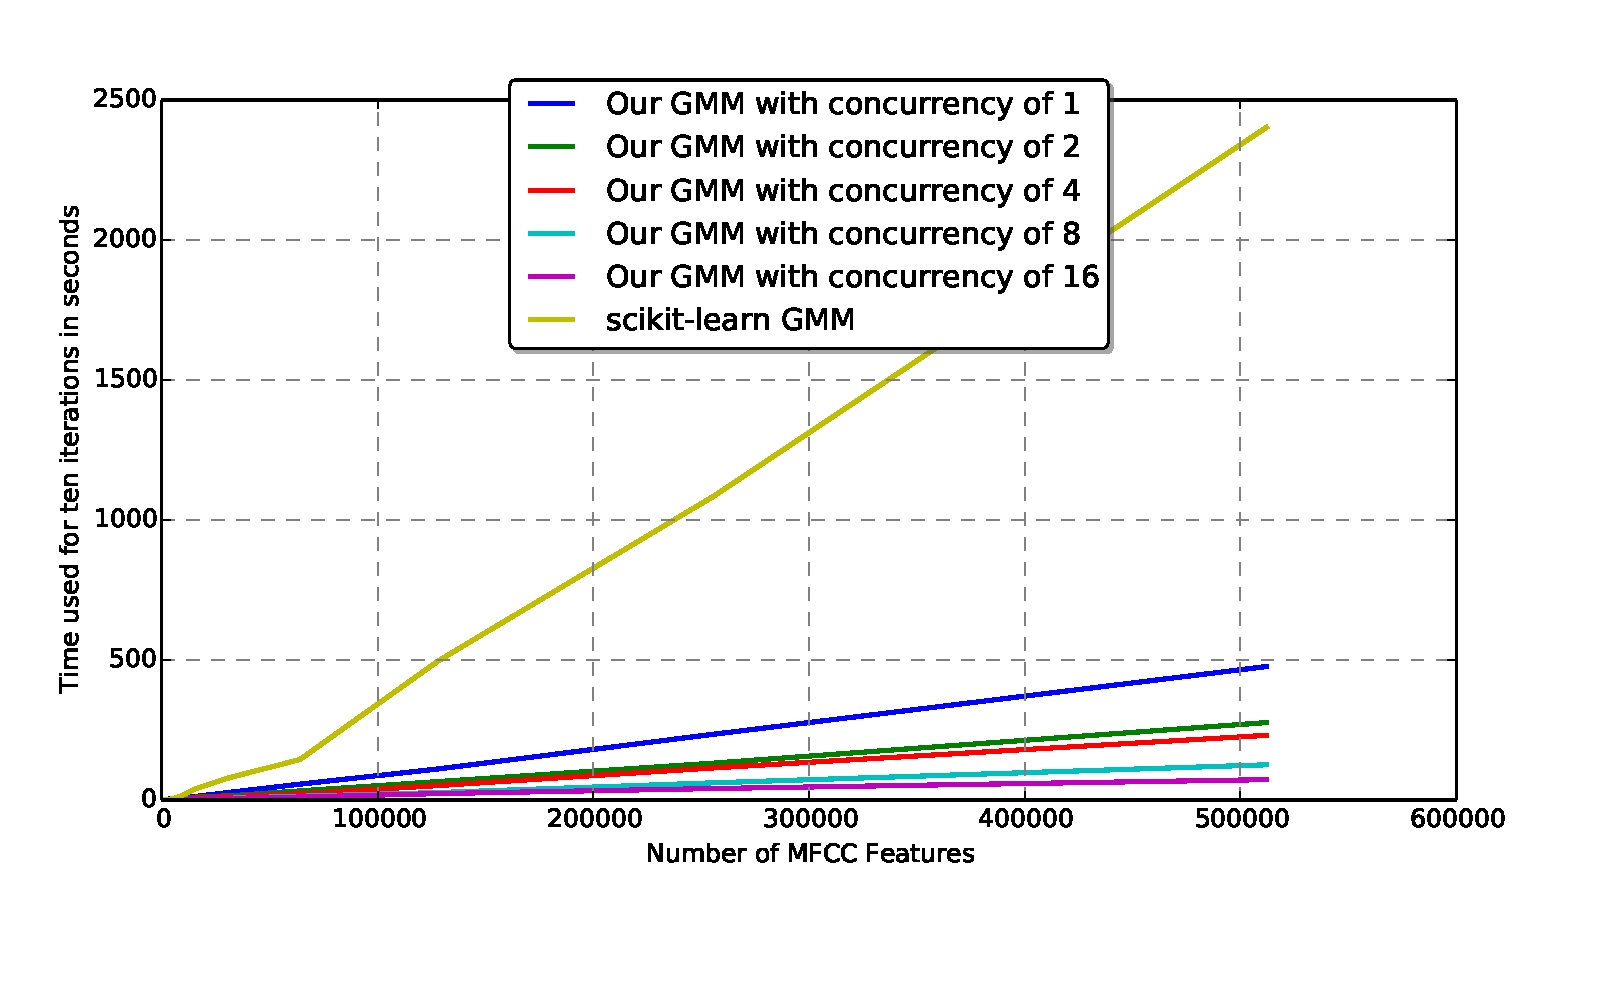
\includegraphics[width=\linewidth]{img/time-comp.pdf}
		\caption{Comparison on efficiency\label{fig:gmm_efficiency}}
	\end{minipage}
	\hfill
	\begin{minipage}{0.48\linewidth}
		\centering
		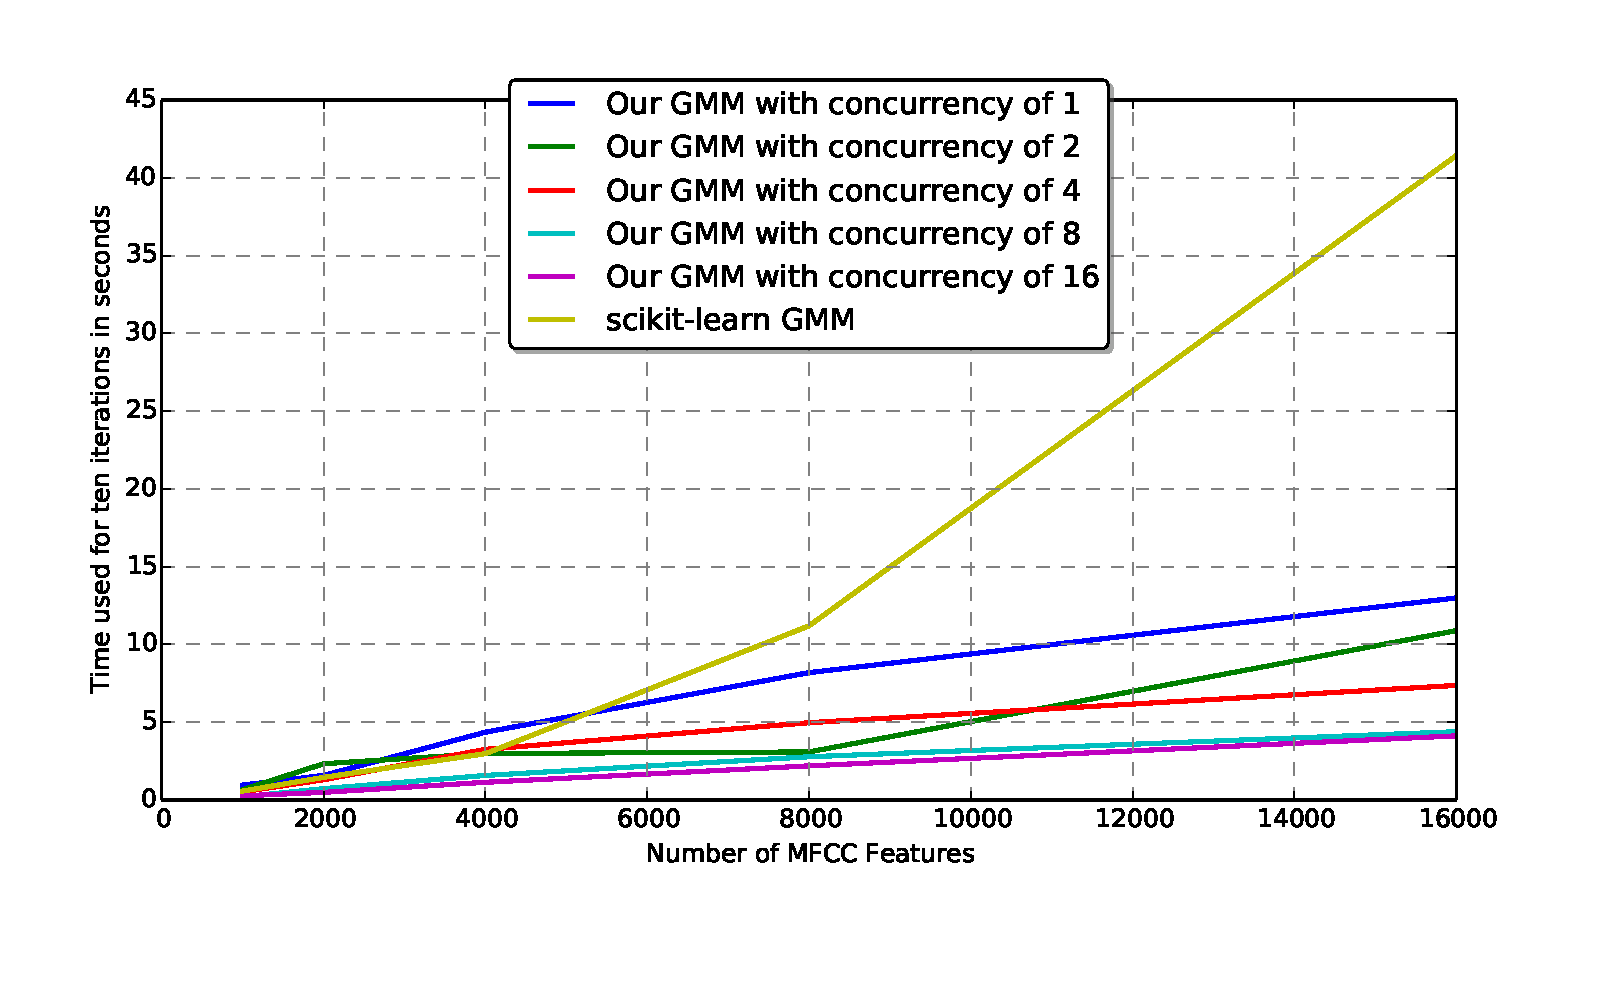
\includegraphics[width=\linewidth]{img/time-comp-small.pdf}
		\caption{Comparison on efficiency when number of MFCC features is small\label{fig:gmm_efficiency_small}}
	\end{minipage}
\end{figure}

From \figref{gmm_efficiency}, we can immediately infer that our method
is much-much more efficient than the widely used version of GMM provided
by scikit-learn when the data size grows sufficiently large.

We shall analyze in two aspect:
\begin{itemize}
    \item No concurrency

             When the number of MFCC features grows sufficiently large, our method
                shows great improvement. When training 512,000 features, our method
                is 5 times faster than comparing method.
    \item With concurrency \\
        Our method shows considerable concurrency scalability that the running time
        is approximately lineary to the number of cores using.

        When using 8-cores, our method is \textbf{$19$ times} faster than comparing
        method.
\end{itemize}


\subsection{Change in MFCC Parameters}
The following tests reveal the effect of MFCC parameters on the final accuracy.
The tests were all performed on ``Style-Reading'' corpus with 40 speakers, each with 20 seconds for enrollment
and 5 seconds for recognition.
\begin{enumerate}
  \item Different Number of Cepstrums
    \begin{figure}[H]
      \centering
      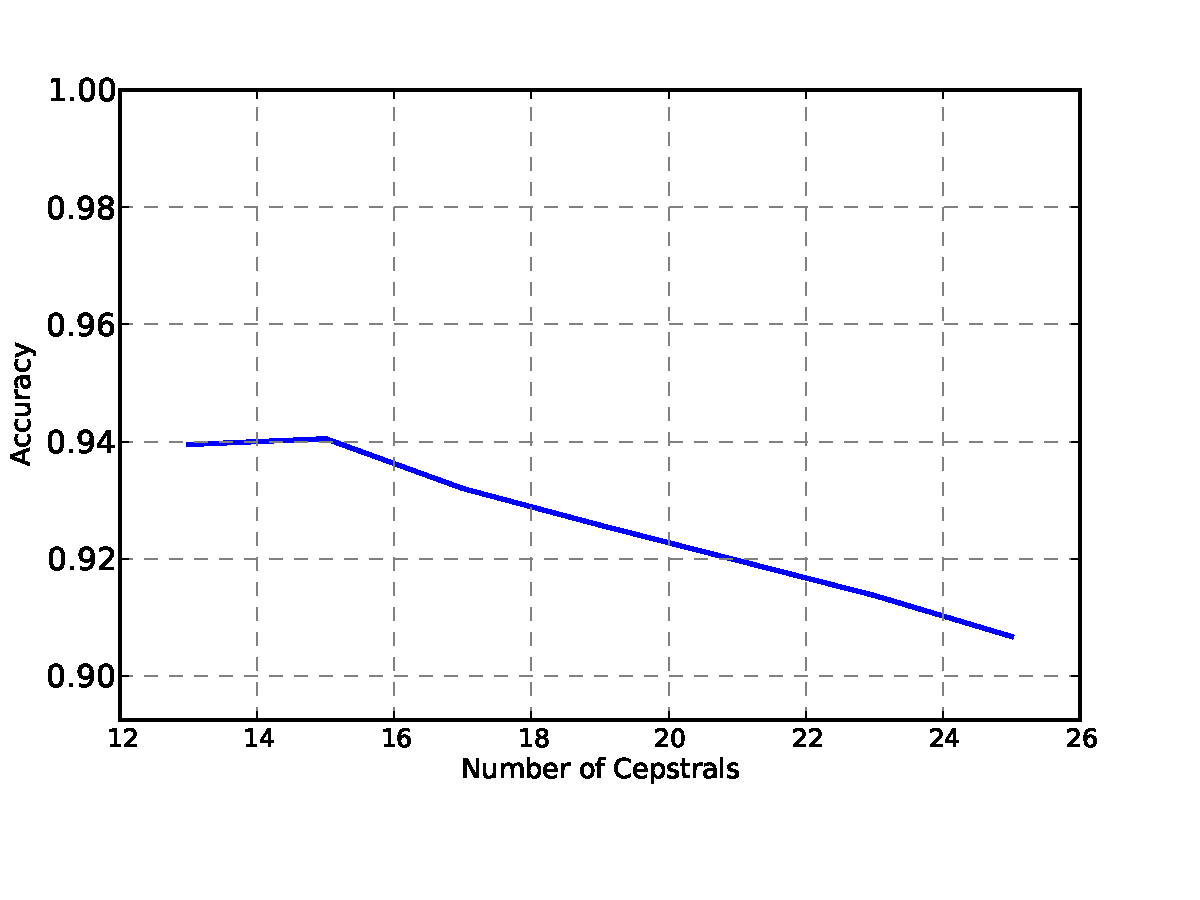
\includegraphics[width=0.7\textwidth]{img/mfcc-nceps.pdf}
    \end{figure}

  \item Different Number of Filterbanks
    \begin{figure}[H]
      \centering
      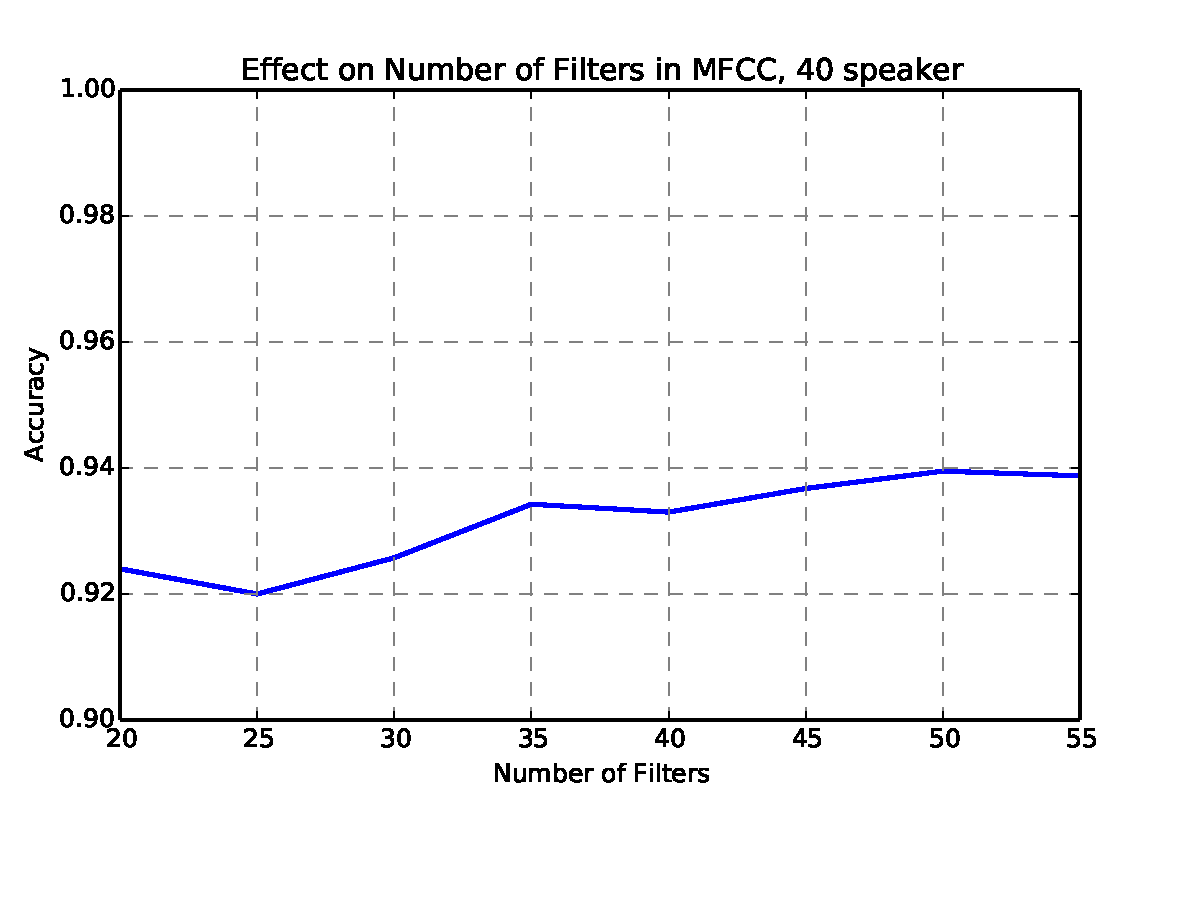
\includegraphics[width=0.7\textwidth]{img/mfcc-nfilter.pdf}
    \end{figure}

  \item Different Size of Frame
    \begin{figure}[H]
      \centering
      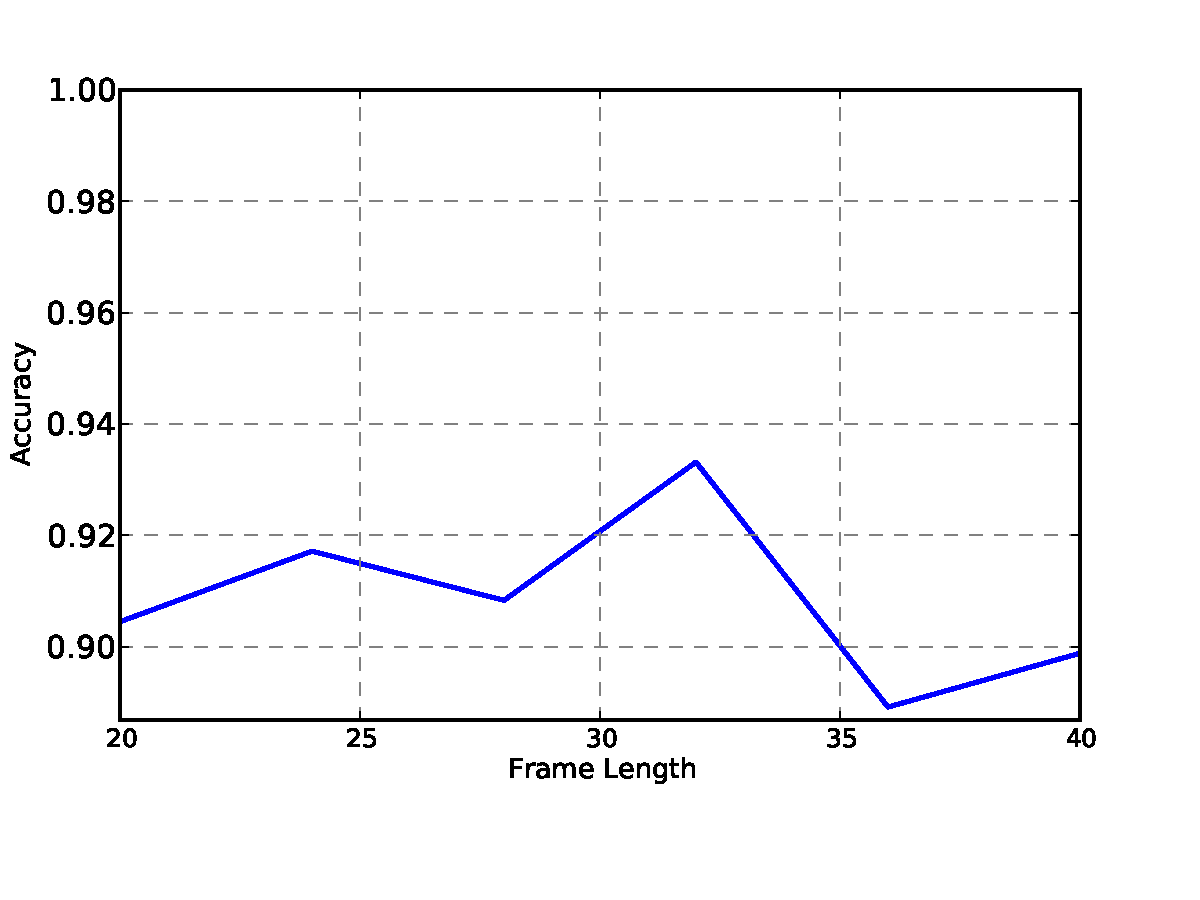
\includegraphics[width=0.7\textwidth]{img/mfcc-frame-len.pdf}
    \end{figure}
\end{enumerate}

\subsection{Change in LPC Parameters}
The following tests display the effect of LPC parameters on the final accuracy.
The tests were performed on ``Style-Reading'' with 40 speakers, each with 20 seconds for enrollment
and 5 seconds for recognition.
\begin{enumerate}
  \item Different Number of Coefficient
    \begin{figure}[H]
      \centering
      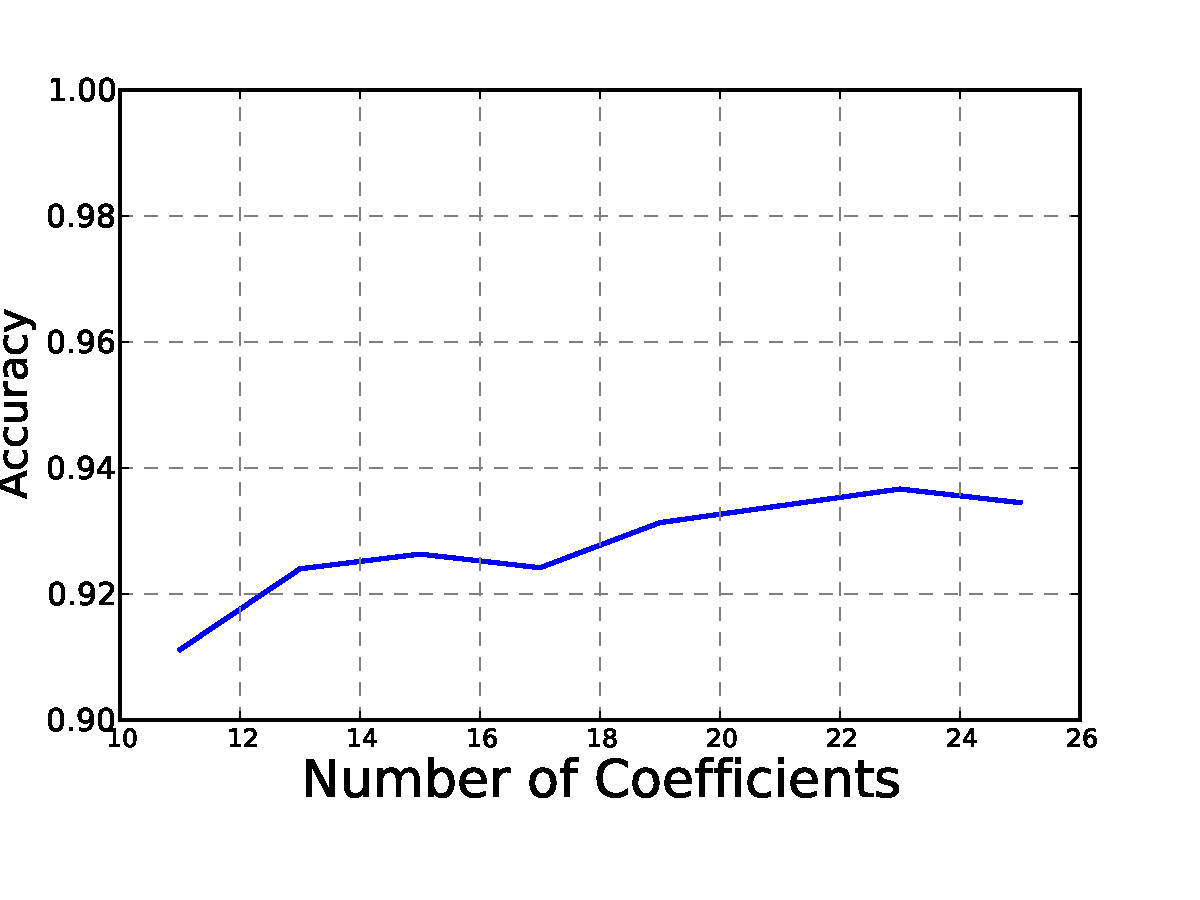
\includegraphics[width=0.7\textwidth]{img/lpc-nceps.pdf}
    \end{figure}

  \item Different Size of Frame
    \begin{figure}[H]
      \centering
      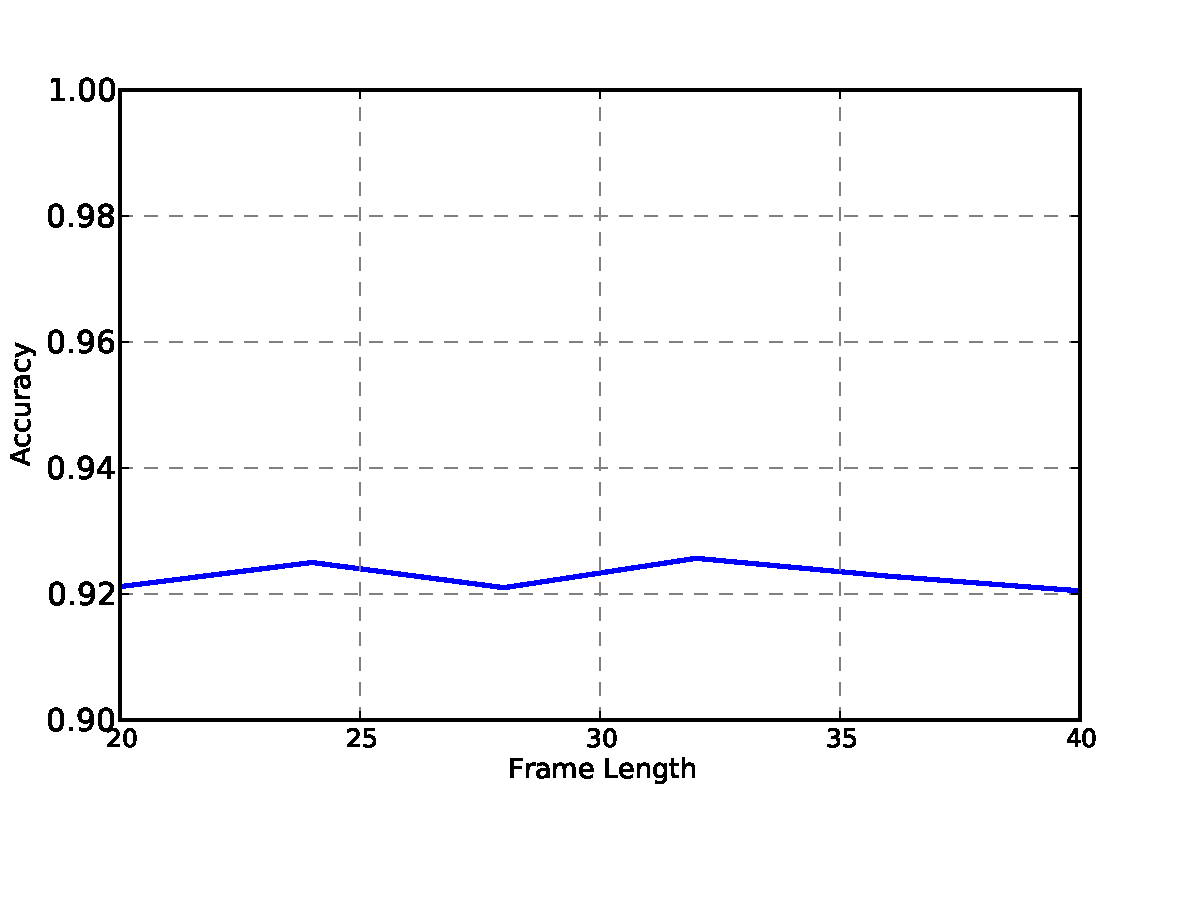
\includegraphics[width=0.7\textwidth]{img/lpc-frame-len.pdf}
    \end{figure}
\end{enumerate}

\subsection{Change in GMM Components}

We experimented on the effect of GMM Components. We found that the number of components
have slight effect on the accuracy, but a GMM with higher order might take
significantly longer time to train. Therefore we still use GMM with 32 components in our system.

\begin{figure}[H]
  \centering
  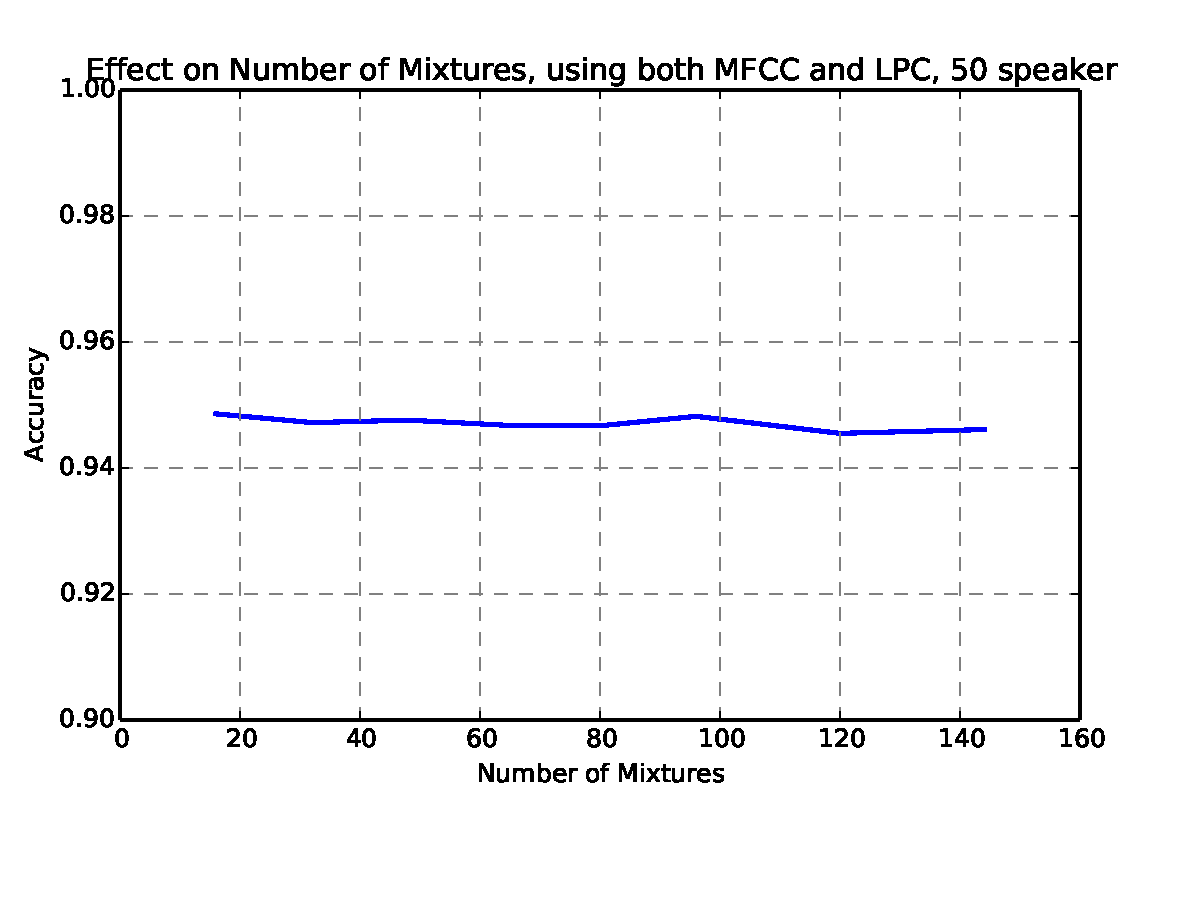
\includegraphics[width=0.7\textwidth]{img/nmixture.pdf}
\end{figure}

\subsection{Different GMM Algorithms}
We compare our implementation of GMM to GMM in scikits-learn.

The configurations of the test is as followed:
\begin{itemize}
    \item Only MFCC: frame size is $20 ms $, 19 cepstrums, 40 filterbanks
	\item Number of mixtures is set to 32, the optimal number we found previously
	\item GMM from scikit-learn, compared to our GMM.
	\item 30s training utterance and 5s test utterance
	\item 100 sampled test utterance for each user
\end{itemize}

\begin{figure}[!ht]
	\centering
	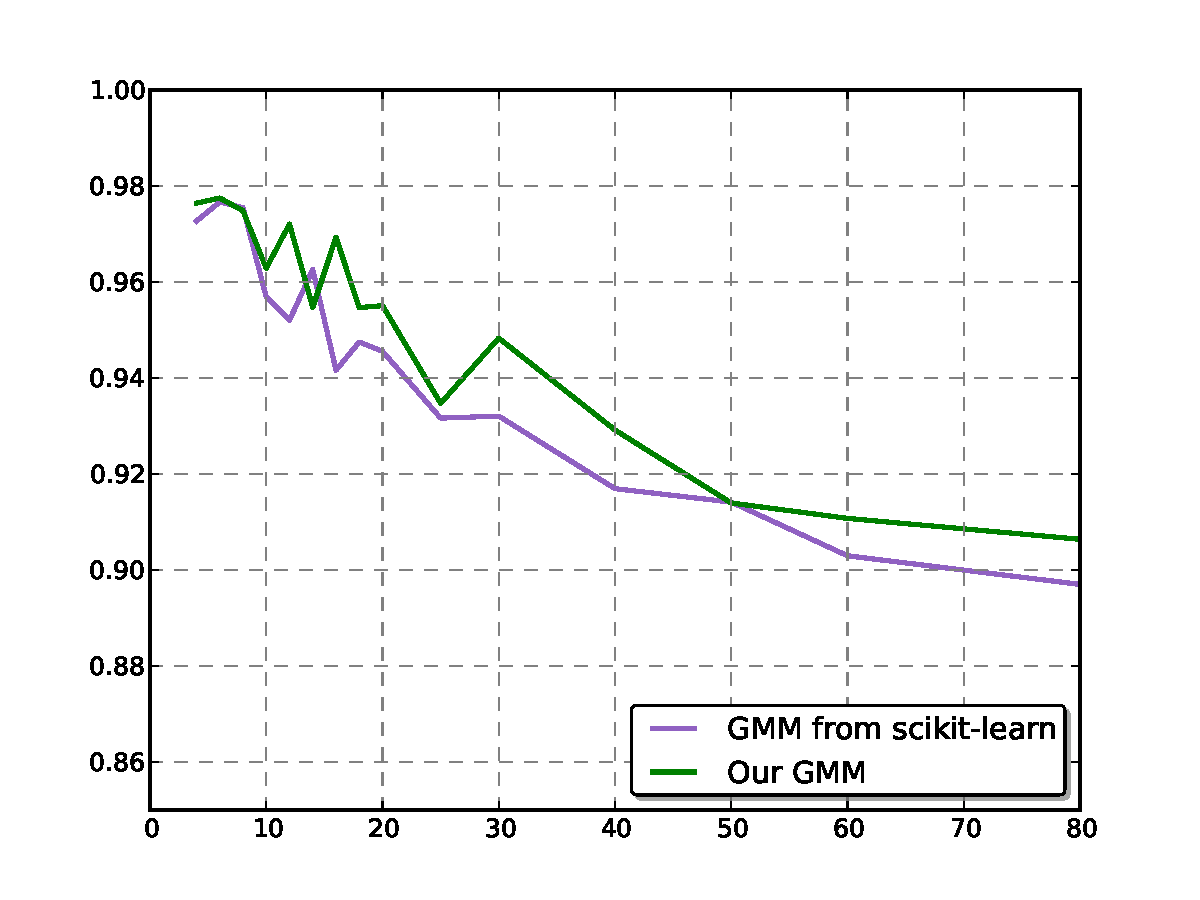
\includegraphics[width=\linewidth]{img/gmm-compare.pdf}
	\caption{Accuracy curve for two GMM}
\end{figure}

From this graph we could see that, our GMM performs better than GMM from scikit-learn in general.
Due to the random selection of test data,
the variance of the test can be high when the number of speakers is small,
as is also the case in the next experiment. But this result still shows that
our optimization on GMM takes effect.

\subsection{Accuracy Curve on Different Number of Speakers}

An apparent trade-off in speaker recognition task is the number of speakers
enrolled and the accuracy on recognization.
Also, the duration of signal for enrollment and test can have significant effect on the accuracy.
We've conducted test using well-tuned parameters for feature extraction as well as GMM, on dataset with
various number of people and with various test duration.

The configurations of this experiment is as followed:
\begin{itemize}
  \item Database: ``Style-Reading''
  \item MFCC: frame size is $32 ms $, 19 cepstrums, 55 filterbanks
  \item LPC: frame size is $32 ms $, 15 coefficients
  \item GMM from scikit-learn, number of mixtures is 32
  \item 20s utterance for enrollment
  \item 50 sampled test utterance for each user
\end{itemize}

\begin{figure}[H]
  \centering
  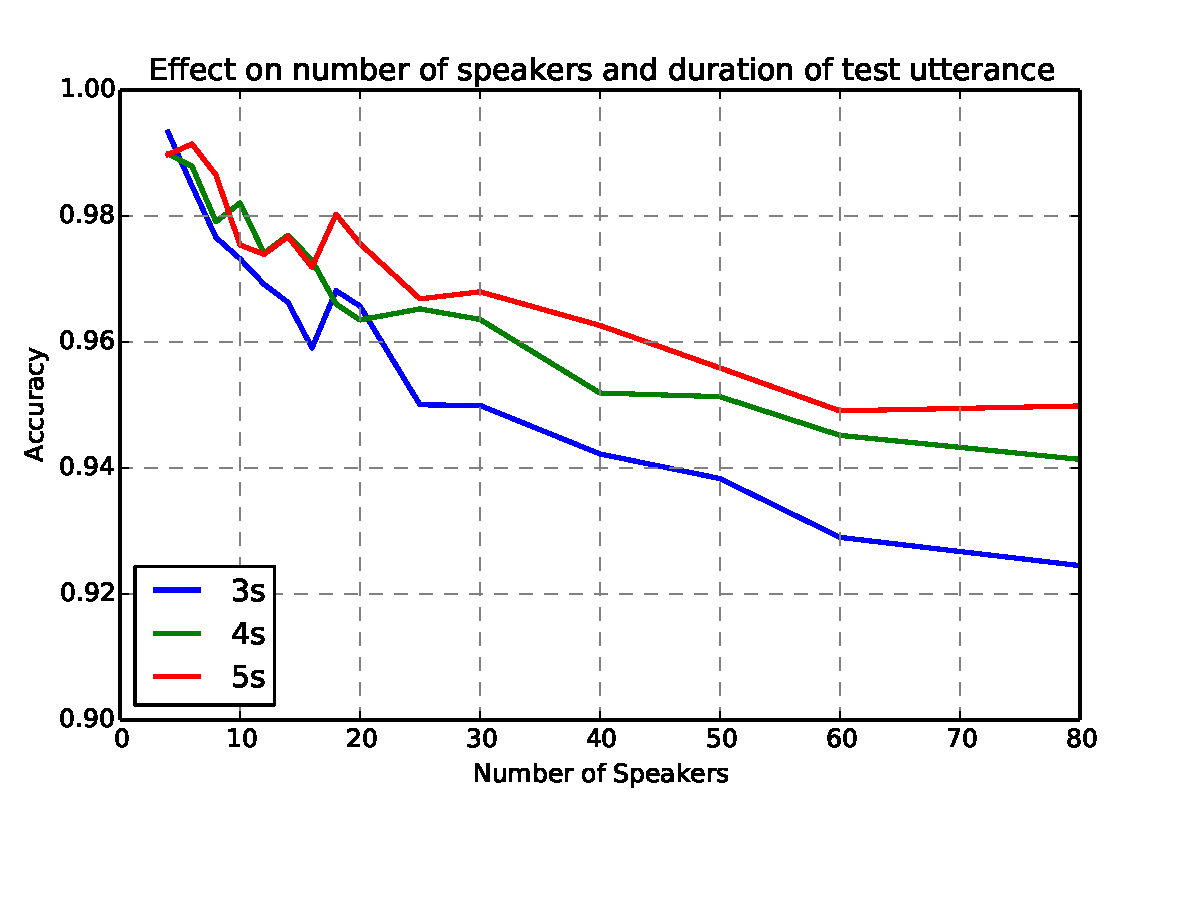
\includegraphics[width=0.8\textwidth]{img/performance.pdf}
\end{figure}

We also conducted experiments on different style of corpus.
The configurations of this experiment is as followed:
\begin{itemize}
  \item MFCC: frame size is $32 ms $, 15 cepstrums, 55 filterbanks
  \item LPC: frame size is $32 ms $, 23 coefficients
  \item GMM from scikit-learn, number of mixtures is 32
  \item 20s utterance for enrollment
  \item 50 sampled test utterance for each user
\end{itemize}

The result is shown below. Note that each point in the graph is an
average value of 20 independent test with random sampled speakers .

\begin{figure}[H]
  \centering
  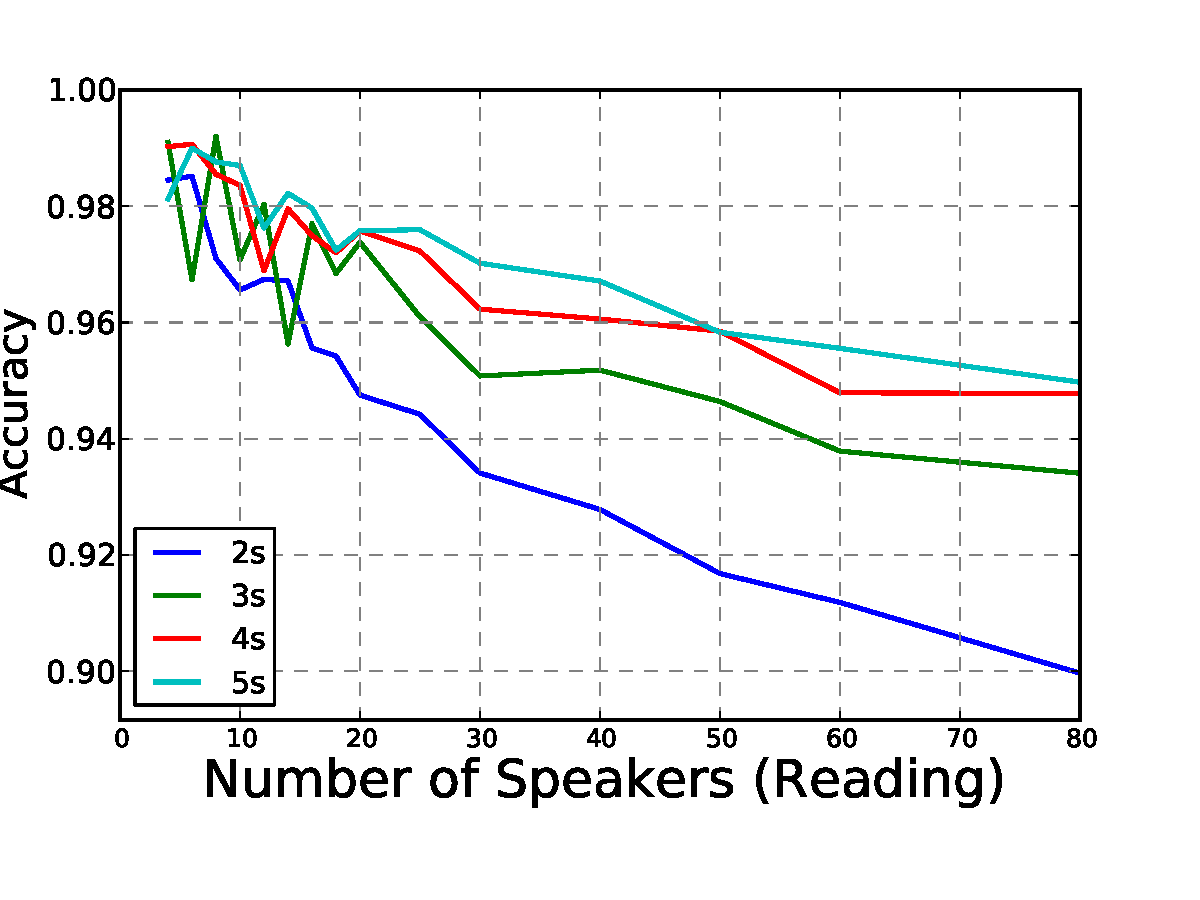
\includegraphics[width=0.8\textwidth]{img/reading.pdf}
\end{figure}
\begin{figure}[H]
  \centering
  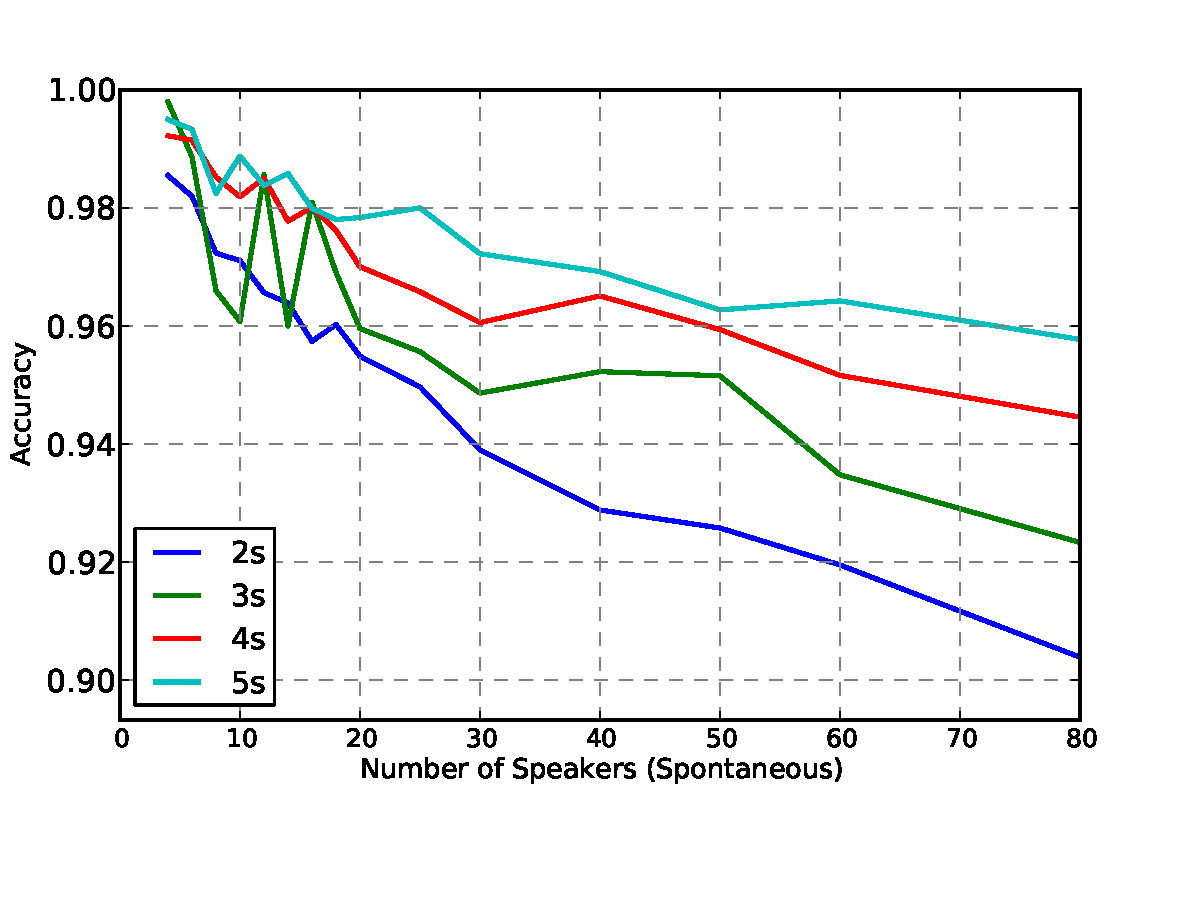
\includegraphics[width=0.8\textwidth]{img/spont.pdf}
\end{figure}

\begin{figure}[H]
  \centering
  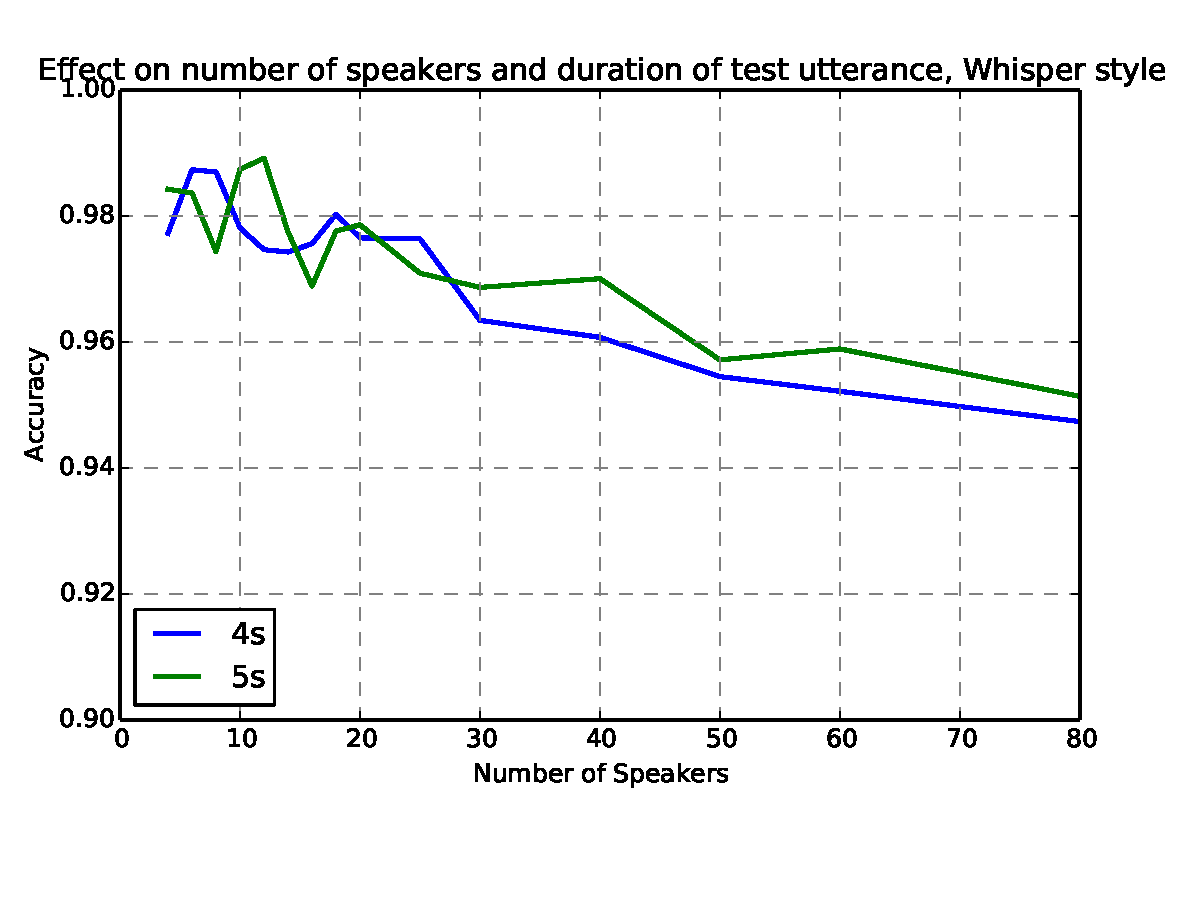
\includegraphics[width=0.8\textwidth]{img/whisper.pdf}
\end{figure}

\subsection{CRBM Performance Test}
We also tested RBM using following configuration:
\begin{itemize}
  \item MFCC: frame size is $32 ms $, 15 cepstrums, 55 filterbanks
  \item LPC: frame size is $32 ms $, 23 coefficients
  \item CRBM with 32 hidden units.
  \item 50 sampled test utterance for each user
  \item 5s test utterance
\end{itemize}

\begin{figure}[H]
  \centering
  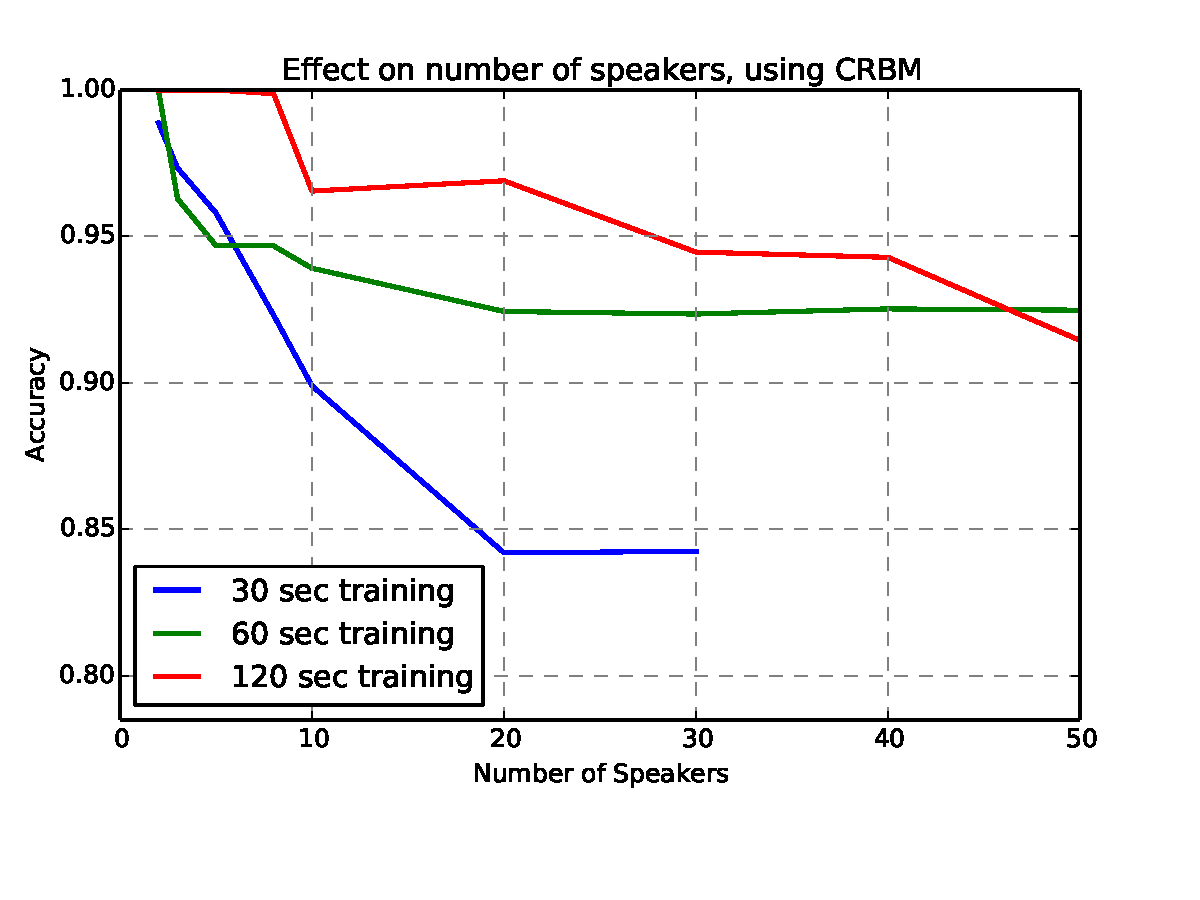
\includegraphics[width=0.9\textwidth]{img/crbm.pdf}
  \caption{\label{fig:crbmresult}}
\end{figure}

Result shown in \figref{crbmresult} indicates that, although CRBM have
generic modeling ability, applying it on signal features does not fit
our expectation. To achieve similar results, the training utterance should
be twice as large as GMM used. Further investigation on using RBM to
process signal features need to be conducted.



\section{GUI}
The GUI contains following tabs:
\begin{itemize}
  \item \textbf{Enrollment} \\

    \begin{figure}[H]
      \centering
      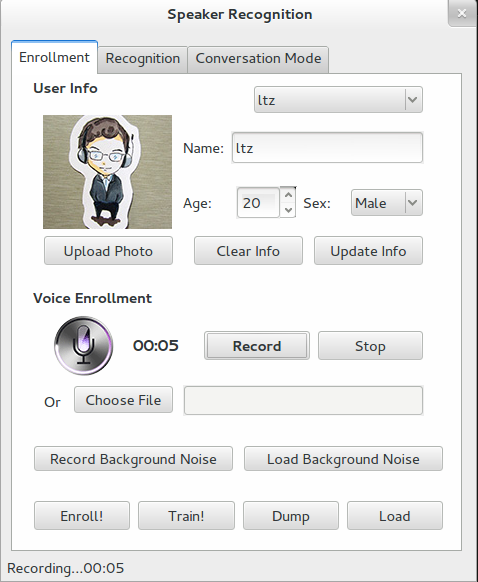
\includegraphics[width=0.8\textwidth]{img/enrollment.png}
    \end{figure}

    A new user may start his or her first step by clicking the
    tab Enrollment. New users could provide personal information
    such as name, sex, and age. then upload personal avatar to
    build up their own data. Experienced users can choose from
    the userlist and update their infomation.

    Next the user needs to provide a piece of utterance for
    the enrollment and training process.

    There are two ways to enroll a user:
    \begin{itemize}
      \item \textbf{Enroll by Recording}
        Click Record and start talking while click Stop to stop
        and save.There is no limit of the content of the utterance,
        whileit is highly recommended that the user speaks long enough
        to provide sufficient message for the enrollment.

      \item \textbf{Enroll from Wav Files}
        User can upload a pre-recorded voice of a speaker.(*.wav recommended)
        The systemaccepts the voice given and the enrollment of a speaker is done.
    \end{itemize}

    The user can train, dump or load his/her voice features after enrollment.

  \item \textbf{Recognition of a user} \\
    \begin{figure}[H]
      \centering
      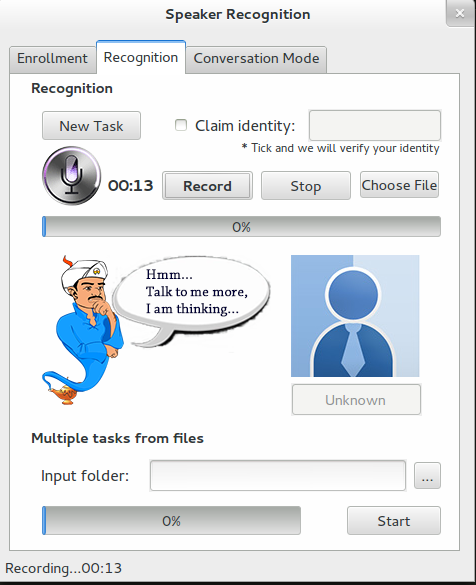
\includegraphics[width=0.8\textwidth]{img/recognition.png}
    \end{figure}

    A enrolled user present or record a piece of utterance,
    the system tells who the person is and show user's avatar.
    Recognition of multiple pre-recorded files can be done as well.

  \item \textbf{Conversation Recognition Mode} \\
    \begin{figure}[H]
      \centering
      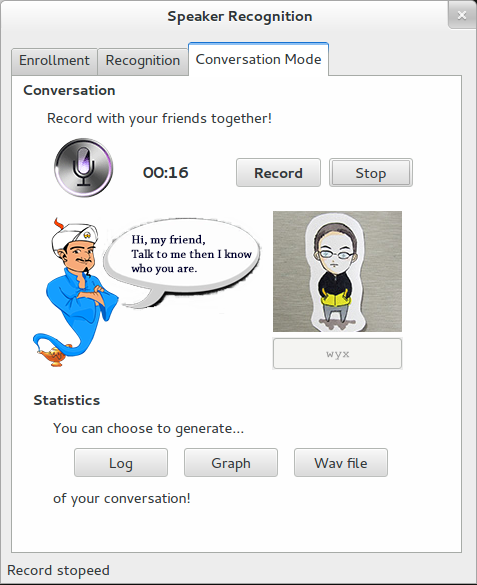
\includegraphics[width=0.8\textwidth]{img/conversation.png}
      \caption{\label{fig:}}
    \end{figure}

    In Conversation Recognition mode, multiple users can have conversations
    together near the microphone. Same recording procedure as above.
    The system will continuously collect voice data, and determine
    who is speaking right now. Current speaker's anvatar will show up
    in screen; otherwise the name will be shown. The conversation
    audio can be downloaded and saved.
    There are some ways to visualize the speaker-distribution in the
    conversation.
    \begin{itemize}
      \item \textbf{Conversation log}
        A detailed log, including start time, stop time,
        current speaker of each period is generated.
      \item \textbf{Conversation flow graph}
        \begin{figure}[H]
          \centering
          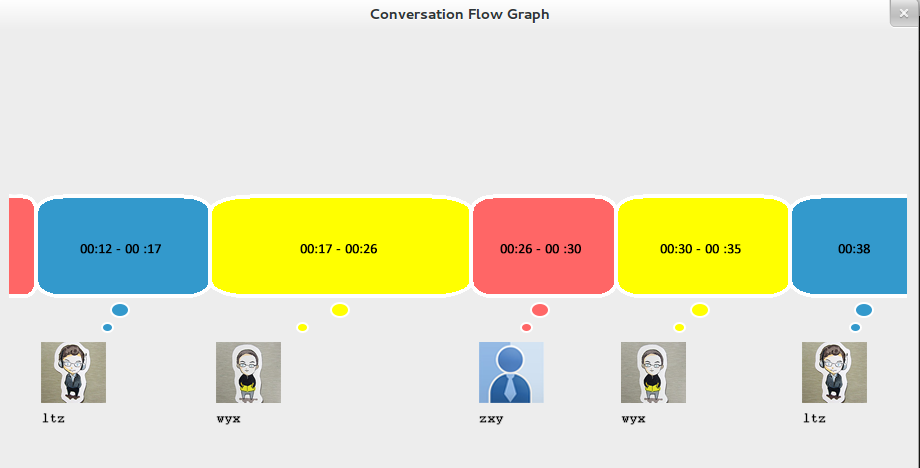
\includegraphics[width=0.8\textwidth]{img/conversationgraph.png}
        \end{figure}

        A timeline of the conversation will be shown by a number of
        talking-clouds joining together, with start time, stop time
        and users' avatars labeled. Different users are presented
        with different colors.The timeline will flow to the left dynamically
        just as time elapses. The visualization of the conversation is done
        in this way. This functionality is still under development.
    \end{itemize}

\end{itemize}


\printbibliography

\end{document}

